\documentclass[11pt,titlepage]{article}
\usepackage{fullpage}
\usepackage{amsmath}
\usepackage{amssymb}
\usepackage{gensymb}
\usepackage[parfill]{parskip}
\usepackage{color}
\usepackage{bm}
\usepackage{graphicx}
\graphicspath{ {images/} }
\usepackage{tikz}
\usetikzlibrary{shapes,arrows,positioning,calc}
\usepackage{float}
\restylefloat{table}
\usepackage{array}
\tikzset{
    block/.style = {draw, fill=white, rectangle, minimum height=3em, minimum width=3em},
    sum/.style = {draw, fill=white, circle, node distance=1cm},
    input/.style = {draw=none},
    output/.style = {draw=none},
    coord/.style = {coordinate}
}

\author{Rane Brown \\ Kate Schneider}
\title{ECEN 4638: Lab W2}
\date{\today}

\begin{document}
\maketitle
\tableofcontents
\listoffigures
\listoftables
\newpage

\section{Description}
	The goal of this lab is to design a controller and investigate the response of a two disc system when using $\omega_1$ for feedback and measurement versus using $\omega_2$. The key difference between these two methods is $\omega_1$ is collocated control while $\omega_2$ is non-collocated. We anticipate using $\omega_1$ will produce a more robust controller and during the course of this lab we will confirm or refute this prediction.

\section{Setup}
	For the following experiments we will arrange the TDS with the lower disc containing four weights at 6.5 cm and the middle disc with two weights at 6.5 cm. Using this setup the system parameters calculated from the methods described in Lab W are the following:
	\begin{align*}
		b &= 0.305 & k &= 2.55\\
		c_1 &= 0.004 & c_2 &= 0.0016\\
		J_1 &= 0.011475 & J_2 &= 0.0064375
	\end{align*}

\section{System model}
	
	\subsection{LTI model}	
		The two disc torsional disc system can be modeled as an LTI system with the following equations:
		\begin{align}
			J_1\ddot \theta_1+c_1\dot \theta_1+k(\theta_1-\theta_2)&=bu \\
			J_2\ddot \theta_2+c_2\dot \theta_2+k(\theta_2-\theta_1)&=0
		\end{align}
		 The difference in position of the discs, $\beta$ is also of interest, where $\beta = \theta_1-\theta_2$. If we make this substitution, as well as substituting in angular velocity $\omega$ for $\dot \theta$, our system becomes:
		 \begin{align}
		 	J_1\dot \omega_1+c_1\omega_1+k\beta=bu \\
			J_2\dot \omega_2+c_2\omega_2-k\beta=0
		 \end{align}
	 
	\subsection{State Space Representation}
		Lab W2 will use the state space representation of the LTI model. State space methods are used because they are easier to manipulate when dealing with a system with multiple outputs such as the two disc TDS.
		\begin{equation}
			\begin{bmatrix}
				\dot \omega_1\\
				\dot \omega_2\\
				\dot \beta
			\end{bmatrix}=
	  		\begin{bmatrix}
	    		-\frac{c_1}{J_1} & 0 & -\frac{k}{J_1} \\
		    	0 & -\frac{c_2}{J_2} & -\frac{k}{J_2}\\
				1 & -1 & 0
	  		\end{bmatrix}
			\begin{bmatrix}
				\omega_1\\
				\omega_2\\
				\beta
			\end{bmatrix}+
			\begin{bmatrix}
				\frac{b}{J_1}\\
				0\\
				0
			\end{bmatrix}
		\end{equation}

\section{Matlab Controller Design $\omega_1$}
	
	\subsection{Specifications $\omega_1$}
		\begin{itemize}
			\item rise time
			\item overshoot
			\item bandwidth
		\end{itemize}

	\subsection{Step Response $\omega_1$}

	\subsection{Frequency Response $\omega_1$}

\section{TDS Controller Implementation $\omega_1$}

	\subsection{Step Response $\omega_1$}

	\subsection{Frequency Response $\omega_1$}

\section{Matlab Controller Design $\omega_2$}

	\subsection{Specifications $\omega_2$}
		The first step in designing a controller that uses $\omega_2$ as the measurement was to select desired system parameters. Based on previous performance of the TDS we decided to select the following parameters.
		\begin{itemize}
			\item rise time $< 1sec$
			\item overshoot $< 15\%$
			\item bandwidth $> 10 \frac{rad}{sec}$
		\end{itemize}

	\subsection{Sisotool}
		After selecting these parameters and entering the system model into Matlab as a state space system we used sisotool to design a notch filter. Matlab's sisotool is very useful because it displays real time results of the controller and the poles and zeros can be adjusted on a root locus plot.
		\begin{figure}[H]
			\centering
			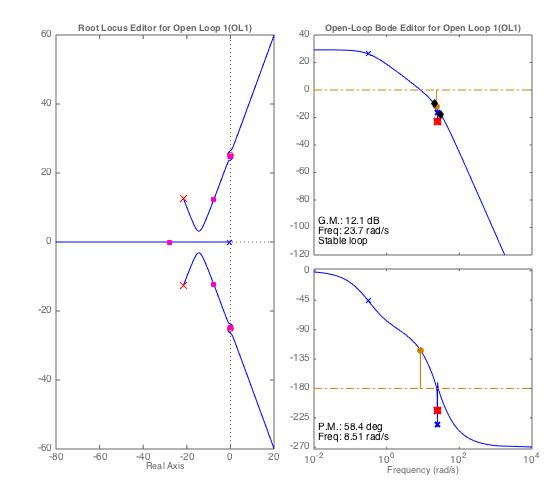
\includegraphics[scale=0.4]{rlocusw2}
			\caption{Root Locus $\omega_2$}
		\end{figure}
		As seen in the root locus plot this system goes unstable if the gain is increased too much. The reason for this is the pole excess in the $H_{u\omega_2}$ transfer function. It is difficult to design a controller that compensates for this excess since it is not possible to create an improper system. Adding additional zeros to the controller helps to stabilize the system but this would require being able to detect the future which is not possible.

	\subsection{Step Response $\omega_2$}
		The below figure shows the step response of the closed loop system when using the $\omega_2$ notch filter controller. This controller provides the following specifications:
		\begin{align*}
			\mbox{RiseTime: } &0.1512 & \mbox{SettlingTime: } &0.7404 & \mbox{SettlingMin: } &0.8862\\
     		\mbox{SettlingMax: } &1.1231 & \mbox{Overshoot: } &16.2071 & \mbox{Undershoot: } &0\\
     		\mbox{Peak: } &1.1231 & \mbox{PeakTime: } &0.3407 &
        \end{align*}
        The rise time meets the desired rise time of less than 1 second but the overshoot is slightly higher than desired. This is a compromise that we are willing to make.
		\begin{figure}[H]
			\centering
			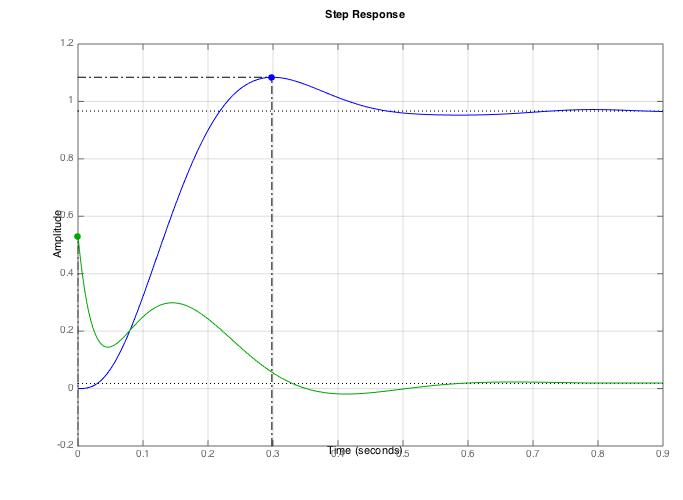
\includegraphics[scale=0.4]{stepw2}
			\caption{Step Response $\omega_2$}
		\end{figure}

	\subsection{Frequency Response $\omega_2$}
		From the bode plot we can see the system will have a relatively low bandwidth but it should meet our design requirements. There is also a section where the higher order system causes an undesirable peak. This could be further reduced with more controller iterations. Using Matlab we calculated the bandwidth to be 14.0037 rad/sec.
		\begin{figure}[H]
			\centering
			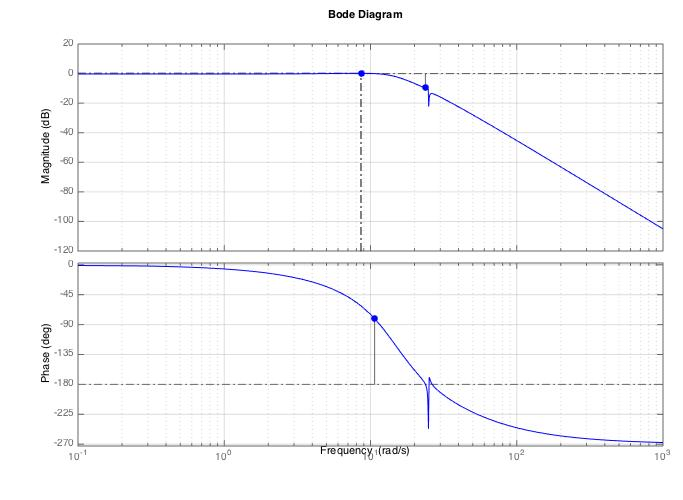
\includegraphics[scale=0.4]{bodew2}
			\caption{Bode Plot $\omega_2$}
		\end{figure}

\section{TDS Controller Implementation $\omega_2$}
	After designing a controller using Matlab and viewing the ideal response values we tested the controller on the TDS system. There were two objectives during the tests. The first objective was to collect information on the step response using the $\omega_2$ controller. The second objective was to collect frequency information using a sinusoidal input in order to reconstruct an experimental bode plot to view the frequency response of the system.

	\subsection{Step Response $\omega_2$}
		The step response data using the designed controller is listed below:
		\begin{align*}
			\mbox{RiseTime: } &1.6716 & \mbox{SettlingTime: } &9.9858 & \mbox{SettlingMin: } &-0.7918\\
     		\mbox{SettlingMax: } &0.9590 & \mbox{Overshoot: } &354.2889 & \mbox{Undershoot: } &4.2572e+03\\
     		\mbox{Peak: } &7.4199 & \mbox{PeakTime: } &6.4500 &
     	\end{align*}
     	\begin{figure}[H]
			\centering
			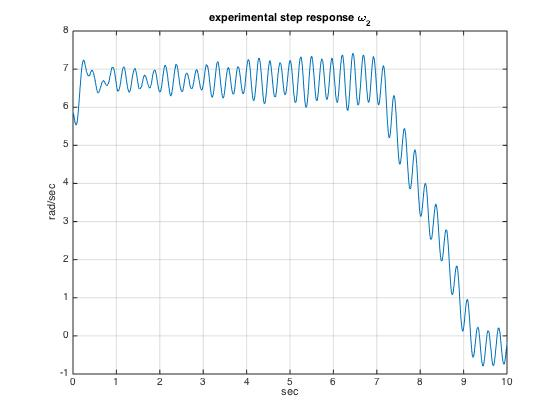
\includegraphics[scale=0.5]{experStepw2}
			\caption{Experimental Step Response $\omega_2$}
		\end{figure}
		It can be seen near the end of the step response that the system is beginning to go unstable. Obviously, this is undesirable but we were unable to design a controller to compensate for this reaction.

	\subsection{Frequency Response $\omega_2$}
		In order to reconstruct a bode plot for the $\omega_2$ controller it was necessary to collect data at multiple frequencies. We collected data at 1,2,3,4,5 hertz. This data was then processed in Matlab to create the below bode plot.
		\begin{figure}[H]
			\centering
			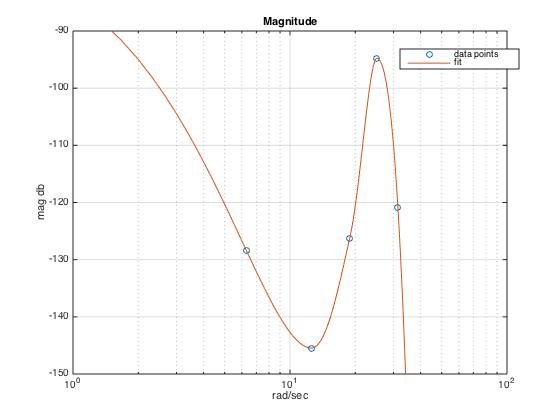
\includegraphics[scale=0.5]{experBodew2}
			\caption{Experimental Step Response $\omega_2$}
		\end{figure}
		Collecting data for more frequencies would provide a much more accurate bode plot but this is a fair representation of the important features of the frequency response.

\section{Controller Comparison}

\end{document}